\chapter{Deployment}
\label{Deployment}
\section{Introduction}
In the following chapter, there is a walk-through on one of many ways to set up a secure pipeline. The pipeline starts with a source code, which will be explained further, and goes on with pushing the code to GitHub and further to \acrshort{aws}. Within these steps are the security measures and scans discussed previously. Some of these steps are automated using Terraform\footnote{Available at: https://www.terraform.io/}, which is a \gls{infrastructure as code} tool. The group has found this repository to be a valuable resource \cite{aws-cicd-pipeline} and used Terraform AWS Documentation\footnote{Available at: https://registry.terraform.io/providers/hashicorp/aws/latest} for information on how to set up the different steps using Terraform. 
\\~\\
Below is a figure of the actual pipeline in \acrshort{aws}, showing its structure and how it is connected together. We will go through the model starting from Git in this chapter.

\vspace{2mm}
\begin{figure}[H]
    \centering
    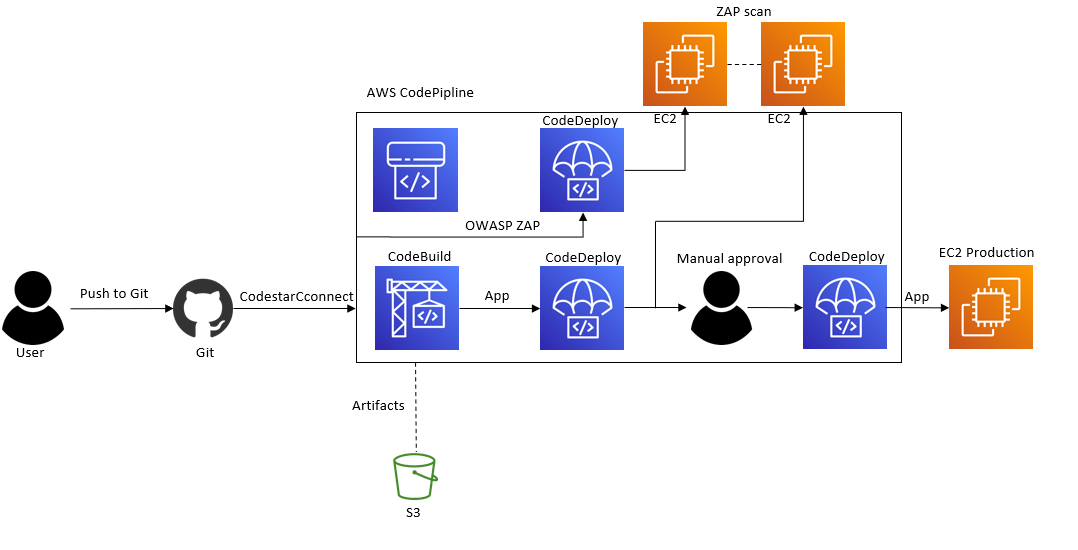
\includegraphics[width=0.8\columnwidth]{Images/aws-piplin-7.png}
    \caption{Pipline in AWS}
    \label{fig: Pipeline in AWS}
\end{figure}



\section{Code used in the pipeline}
For testing the group decided on using OWASPs Juice Shop\footnote{Code available at: https://github.com/juice-shop/juice-shop}, which is a deliberately vulnerable web application that is designed to help developers and others learn about web applications security concepts. The code is designed to simulate a real-world application by having common vulnerabilities within the code. The intention is to encourage users to find these vulnerabilities and exploit them and increase the understanding of web application security \cite{owaspJuiceShop}.
The code in the OWASP Juice Shop is open source code on GitHub and is written in TypeScript, which uses a Node.js server and Angular for \gls{front-end} \cite{owaspJuiceShopCode}.
The code contains different vulnerabilities, including SQL injections, cross-site scripting, and many others. 
Overall, OWASP Juice Shop encourages users to improve their skills and it allows for customization and adaption for specific needs from the users. 

\section{Pushing to GitHub}
When the source code is ready to be pushed to GitHub, security measures must be in place. One of the previously mentioned measurements is branch protection. Branch protection rules are easy to enable in GitHub. It is done for each individual repository. GitHub has different rules one can enable, which are explained in \ref{branchprotection}. This can either be done in \gls{GUI} or automated using Terraform, which is shown in Appendix X. 

Further, the commit signature has to be configured. For signing commits in GitHub, one can either use an SSH or GPG key. These need to be generated and connected to the user's GitHub account.
GitHub provides documentation\footnote{Available at: https://docs.github.com/en/authentication/managing-commit-signature-verification/signing-commits} on how to create a GPG and SSH key, as well as how to connect these keys to a GitHub account.

\begin{figure}[H]
  \centering
  \begin{subfigure}[H]{0.4\textwidth}
    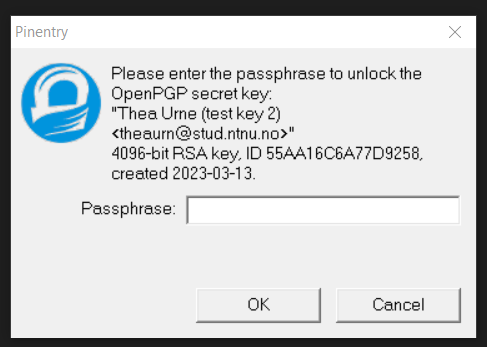
\includegraphics[width=\textwidth]{Images/signedcommits.png}
    \caption{Required passphrase when committing to GitHub}
    \label{fig:image1}
  \end{subfigure}
  \hfill
  \begin{subfigure}[H]{0.4\textwidth}
    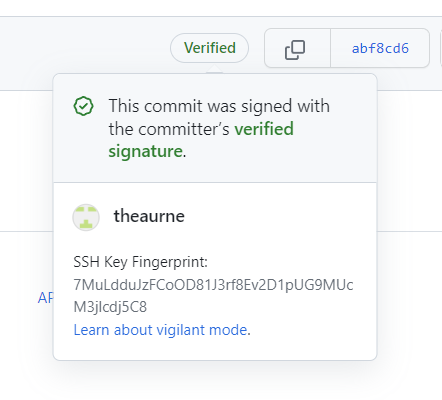
\includegraphics[width=\textwidth]{Images/verified-commit.png}
    \caption{Verified commit}
    \label{fig:image2}
  \end{subfigure}
  \caption{Required signed commits}
  \label{fig:overall}
\end{figure}

\vspace{2mm}
\begin{figure}[H]
    \centering
    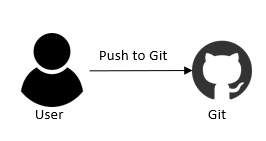
\includegraphics[width=0.5\columnwidth]{Images/aws-piplin-1.png}
    \caption{Pushing to GitHub}
    \label{fig: Pushing to GitHub}
\end{figure}


\section{Managing security in GitHub}
After the source code is pushed to its belonging branch, the code must be scanned for potential vulnerabilities before moving forward. One of these scans is SAST scanning using CodeQL. Setting up CodeQL\footnote{Intructions available at: https://docs.github.com/en/code-security/code-scanning/automatically-scanning-your-code-for-vulnerabilities-and-errors/configuring-code-scanning-for-a-repository} is done by adding the CodeQL YAML file in the workflow. Other security tools in GitHub are Dependabot\footnote{Instructions available at: https://docs.github.com/en/code-security/dependabot/dependabot-security-updates/configuring-dependabot-security-updates} and Secret scanner\footnote{Instructions available at: https://docs.github.com/en/code-security/secret-scanning/configuring-secret-scanning-for-your-repositories}. These are also enabled in the security settings. After being enabled, all these tools automatically scan the code for vulnerabilities.

\begin{figure}[H]
    \centering
    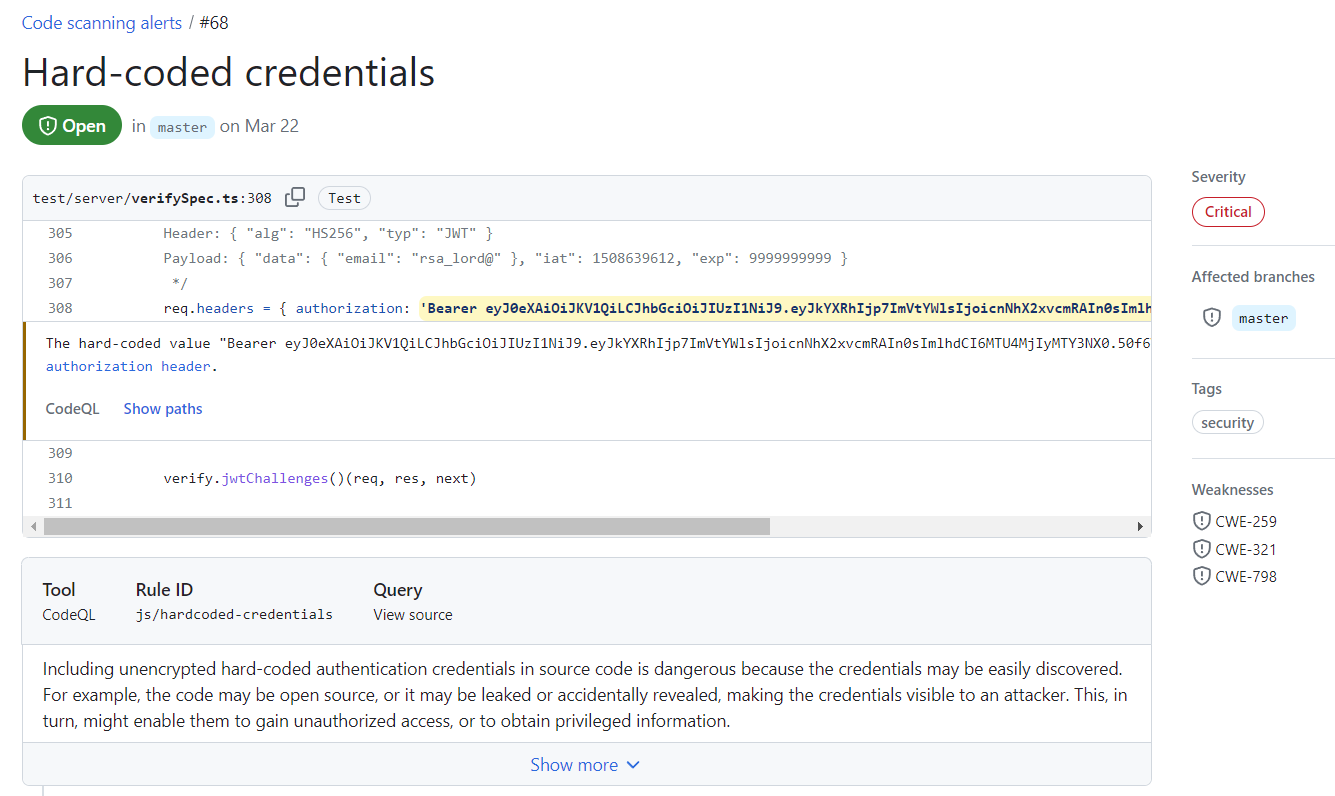
\includegraphics[width=0.8\columnwidth]{Images/codescan.png}
    \caption{Critical alert from code scan}
    \label{fig: Critical alert from code scan}
\end{figure}

An example of code scanning alerts using CodeQL is this critical alert, notifying the user of a hard-coded credential. The code scanning alerts refer to CWE weaknesses, which are explained further in \ref{cwe}.

\vspace{2mm}
\begin{figure}[H]
    \centering
    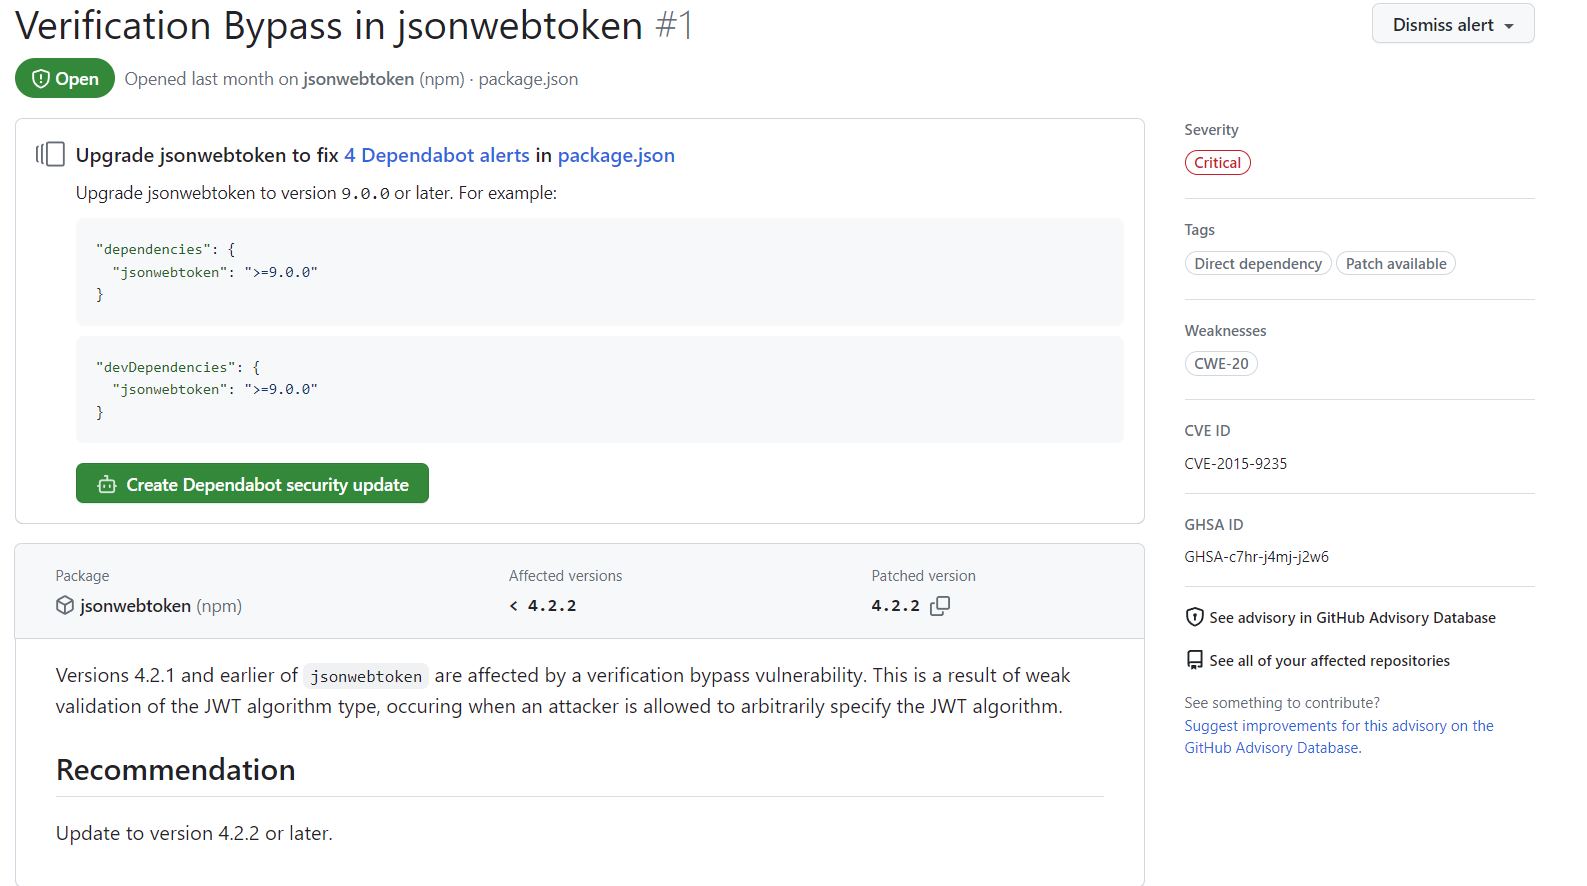
\includegraphics[width=0.8\columnwidth]{Images/dependabotalert.png}
    \caption{Critical alert from Dependabot}
    \label{fig: Critical alert from Dependabot}
\end{figure}

Figure \ref{fig: Critical alert from Dependabot} is one of the critical alerts from Dependabot in the Juice-Shop repository. It shows a vulnerability in the dependency version used, following a suggestion on a patched version. Dependabot, similarly to CodeQL, refers to CWE weaknesses. Additionally, it refers to a CVE ID. 

\vspace{2mm}
\begin{figure}[H]
    \centering
    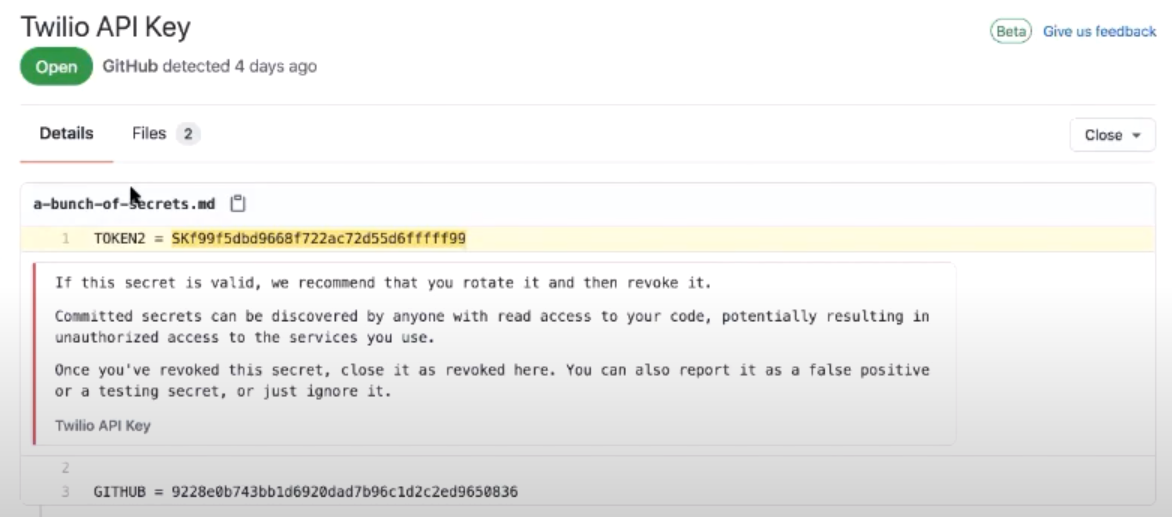
\includegraphics[width=0.8\columnwidth]{Images/secretscanneralert.png}
    \caption{Alert from secret scanner} Adapted from: \cite{GitHubVideo}
    \label{fig: Alert from secret scanner}
\end{figure}
The GitHub Secret scanner did not detect any secrets in the Juice-Shop repository. Therefore, Figure \ref{fig: Alert from secret scanner} is taken from GitHub's demonstration of the secret scanner. The alert warns the user about an API key that matches the pattern of their partner Twilio. 

\section{Committing the source code to AWS}
When all vulnerabilities are detected and fixed in GitHub, the source code can be built in \acrshort{aws}. In order for this to be done, a connection between the \acrshort{aws} and GitHub account needs to be made. AWS CodeStar Connection enables the connection of cloud resources to external code repositories, such as the Juice-Shop repository on GitHub. By creating this connection as a resource, it can be used by \acrshort{aws} CodePipeline to automatically trigger the pipeline in response to any changes made to the GitHub repository.
This can either be done on the \acrshort{aws} website or by using Terraform to create a connection resource with GitHub as the provider. 

\begin{tcolorbox}
\begin{verbatim}
resource "aws_codestarconnections_connection" "code-connection" {
  name          = "code-connection"
  provider_type = "GitHub"
}    
\end{verbatim}
\end{tcolorbox}

Following the successful creation of the connection resource in \acrshort{aws} using Terraform, a manual verification process in \acrshort{aws} is required. This is essential due to the requirement to log in to the system with one's GitHub account credentials, as passing secrets through \acrshort{aws} to GitHub login is not possible, due to the connection opening a third-party login page that \acrshort{aws} does not control.

\vspace{2mm}
\begin{figure}[H]
    \centering
    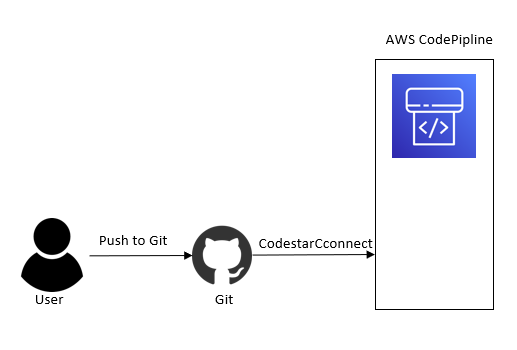
\includegraphics[width=0.6\columnwidth]{Images/aws-piplin-2-1.png}
    \caption{Committing the source code to AWS}
    \label{fig: Committing the source code to AWS}
\end{figure}

\section{Storing artifacts}
To store \gls{artifact}s generated during different stages of the pipeline, an S3 bucket is created. The bucket is created as a resource with optional variables. One crucial aspect to consider is the need for unique bucket names within the server area, as \acrshort{aws} uses this as a means to differentiate between buckets owned by different users. Either the name can be configured like in the code below, or the name variable can be excluded and \acrshort{aws} will configure the name themselves.

\begin{tcolorbox}
\begin{verbatim}
resource "aws_s3_bucket" "codepipeline_artifact" {
  bucket = "artifact-bucket-unique-name"
}
\end{verbatim}
\end{tcolorbox}

In order for each stage to be able to access the S3 bucket and retrieve the last stage's \gls{artifact}s, it has to be given access to the bucket. These access rights have to be individually given to each stage in the pipeline. In the following code the pipeline and every stage are given access to the bucket, hence the "s3:*".

\begin{tcolorbox}
\begin{verbatim}
statement {
    sid       = ""
    actions   = ["s3:*", "codebuild:*"]
    resources = ["*"]
    effect    = "Allow"
}
\end{verbatim}
\end{tcolorbox}

\vspace{2mm}
\begin{figure}[H]
    \centering
    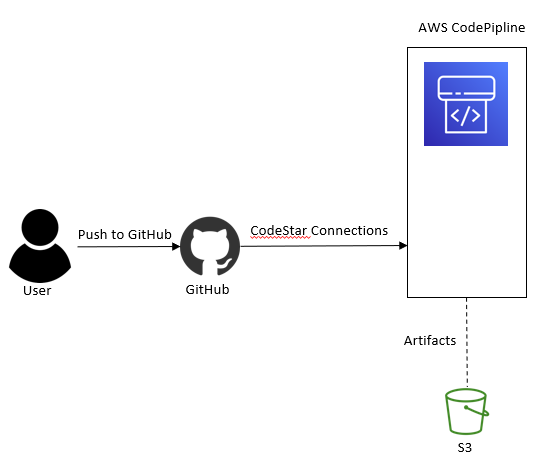
\includegraphics[width=0.6\columnwidth]{Images/aws-piplin-2.png}
    \caption{Storing the artifacts}
    \label{fig: Storing the artifacts}
\end{figure}

\section{Build stage}
In the build stage, CodePipeline uses CodeBuild to compile the source code into a working website. CodeBuild uses a \say{build project} that is created using the code in Appendix X. This build project is used to create the \say{build environment}, which is what operating system, Docker image, and compute- resources and types are used.  It is possible to choose from various compute- environments and types\footnote{Available at: https://docs.aws.amazon.com/codebuild/latest/userguide/build-env-ref-compute-types.html}. In this example, the environment type is set to be a Linux container. The compute type refers to the amount of memory, CPUs, and disk space needed, which in this case is set to be the smallest amount. 

\begin{tcolorbox}
\begin{verbatim}
environment {
    compute_type                = "BUILD_GENERAL1_SMALL"
    image                       = "aws/codebuild/standard:6.0"
    type                        = "LINUX_CONTAINER"
    image_pull_credentials_type = "CODEBUILD"
  }
\end{verbatim}
\end{tcolorbox}

Further, the build project downloads the source code and uses build commands, found in the \gls{buildspec} file, to run the build. The source code is retrieved from the S3 bucket, where it was put from the previous stage. \cite{CodeBuildProcess}

\vspace{2mm}
\begin{figure}[H]
    \centering
    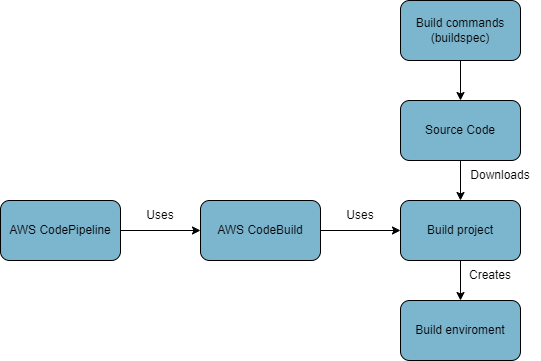
\includegraphics[scale=0.4]{Images/CodeBuild.drawio.png}
    \caption{AWS CodeBuild} 
    \label{fig: AWS CodeBuild}
\end{figure}

\vspace{2mm}
\begin{figure}[H]
    \centering
    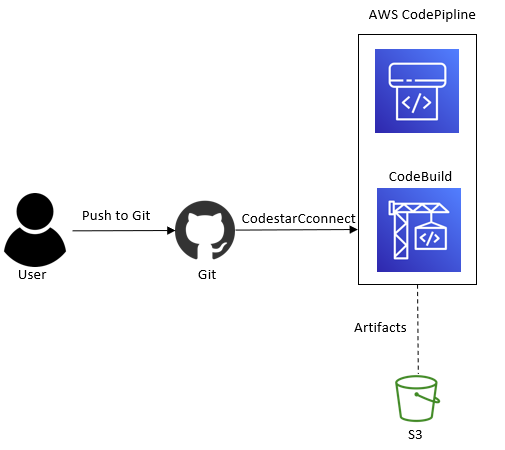
\includegraphics[width=0.6\columnwidth]{Images/aws-piplin-3.png}
    \caption{Build stage}
    \label{fig: Build stage}
\end{figure}

\section{Deployment and Testing}
\label{Deployment and Testing}
Application refers to deployment group and deployment etc (keep track of everything).
The deployment group specifies what configurations to use for the deployment. Also specifies what instance (preconfigured) to use for the deployment.
Deployment deploys the given revision (source code). Appspec is added to the revision. Glossary for appspec.

\vspace{2mm}
\begin{figure}[H]
    \centering
    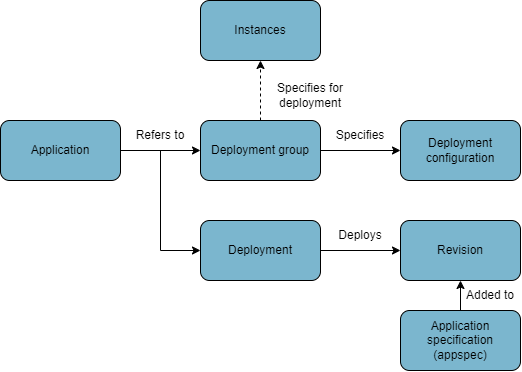
\includegraphics[width=0.6\columnwidth]{Images/CodeDeploy.drawio.png}
    \caption{AWS CodeDeploy}
    \label{fig: AWS CodeDeploy}
\end{figure}

\vspace{2mm}
\begin{figure}[H]
    \centering
    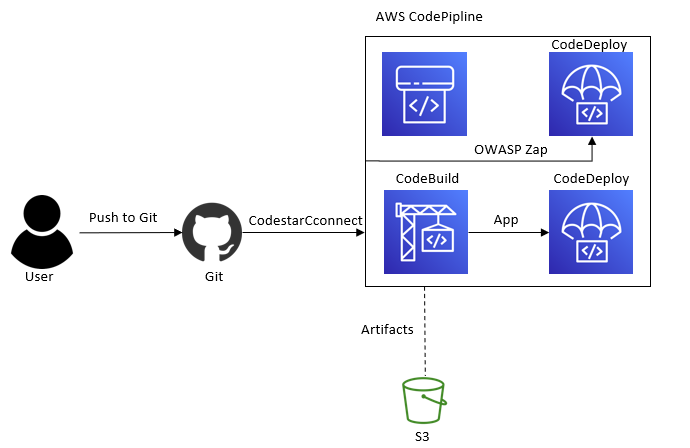
\includegraphics[width=0.6\columnwidth]{Images/aws-piplin-4.png}
    \caption{CodeDeploy}
    \label{fig: CodeDeploy}
\end{figure}


Our security tests work by setting up a Docker container \footnote{https://www.docker.com/resources/what-container/} on this \acrshort{ec2} instance, which uses the weekly stable image \footnote{https://www.zaproxy.org/docs/docker/} of OWASP Zap to run one of the automated standard tests that are predefined by OWASP. Typically, you would build these specifically for your application, but for our demo/test, this works very well. We start up the container and point the scan towards the other instance in our \acrshort{vpc}. This wil give us a resolt lucking like this
\vspace{2mm}
\begin{figure}[H]
    \centering
    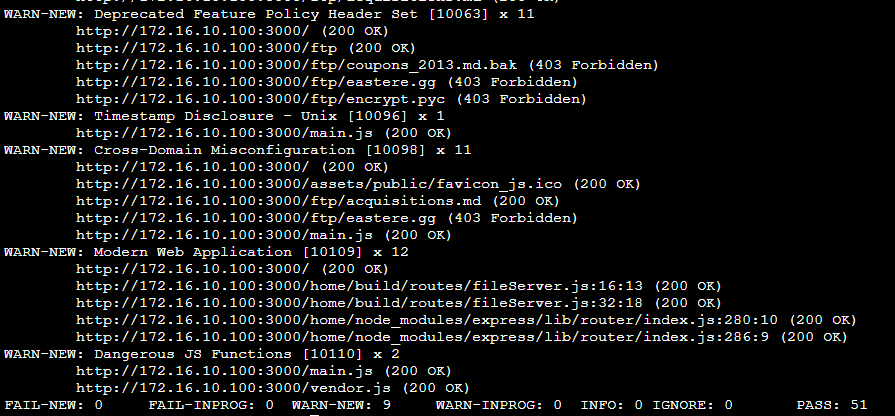
\includegraphics[width=0.8\columnwidth]{Images/owasp-zap-scan.png}
    \caption{OWASP Zap baseline scan}
    \label{fig: OWASP Zap baseline scan}
\end{figure}


To ensure that the to \acrshort{ec2} instances can communicate with each other in the \acrshort{vpc}, we have assigned each instance its own network interface having only one possible IP address. This approach ensures that both instances are always able to locate each other.


\begin{tcolorbox}
\begin{verbatim}
resource "aws_network_interface" "interface_network1" {
  subnet_id   = aws_subnet.my_subnet.id
  private_ips = ["172.16.10.100"]
}

resource "aws_network_interface" "interface_network2" {
  subnet_id   = aws_subnet.my_subnet.id
  private_ips = ["172.16.10.101"]
}
\end{verbatim}
\end{tcolorbox}

\vspace{2mm}
\begin{figure}[H]
    \centering
    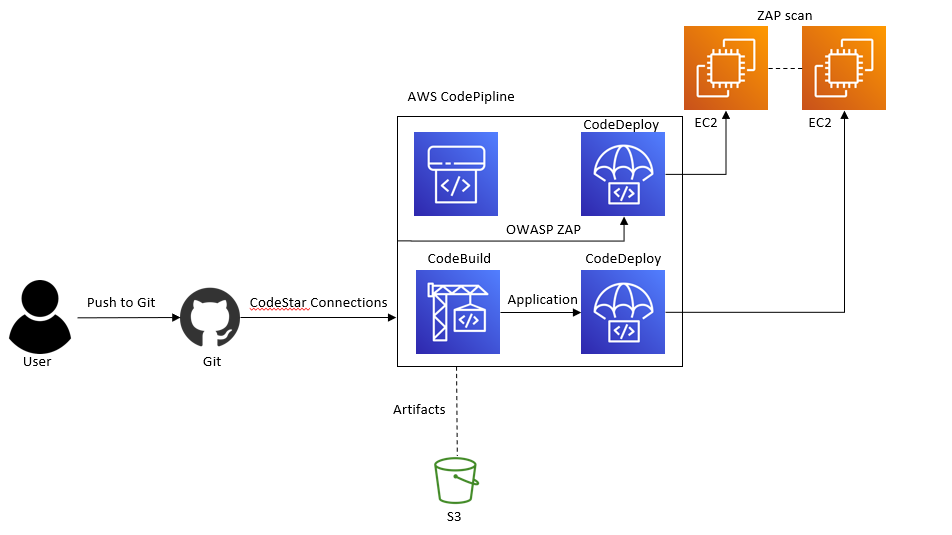
\includegraphics[width=0.7\columnwidth]{Images/aws-piplin-5.png}
    \caption{Depeploy to EC2 and scans the app}
    \label{fig: Depeploy to EC2 and scans the app}
\end{figure}


\section{production}

In the production stage, the CodePipeline uses CodeDeploy to deploy an EC2 instance like we did in the previus chapter, that will host the final product. But before we get to that stage, you need to manually approve the pipeline before the code continues to production. This is so that you can review the results that come from the automated security tests to ensure that you do not deploy faulty code.
\vspace{2mm}
\begin{figure}[H]
    \centering
    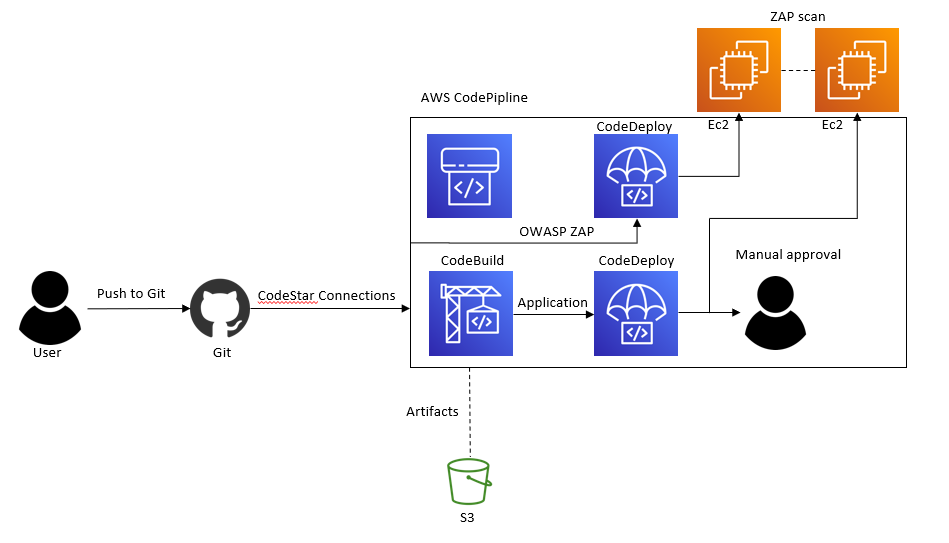
\includegraphics[width=0.8\columnwidth]{Images/aws-piplin-6.png}
    \caption{Manual approval}
    \label{fig: Manual approval}
\end{figure}

After the manual approval is completed, the code will be put into production in the same way that we did in \ref{Deployment and Testing} 
\vspace{2mm}
\begin{figure}[H]
    \centering
    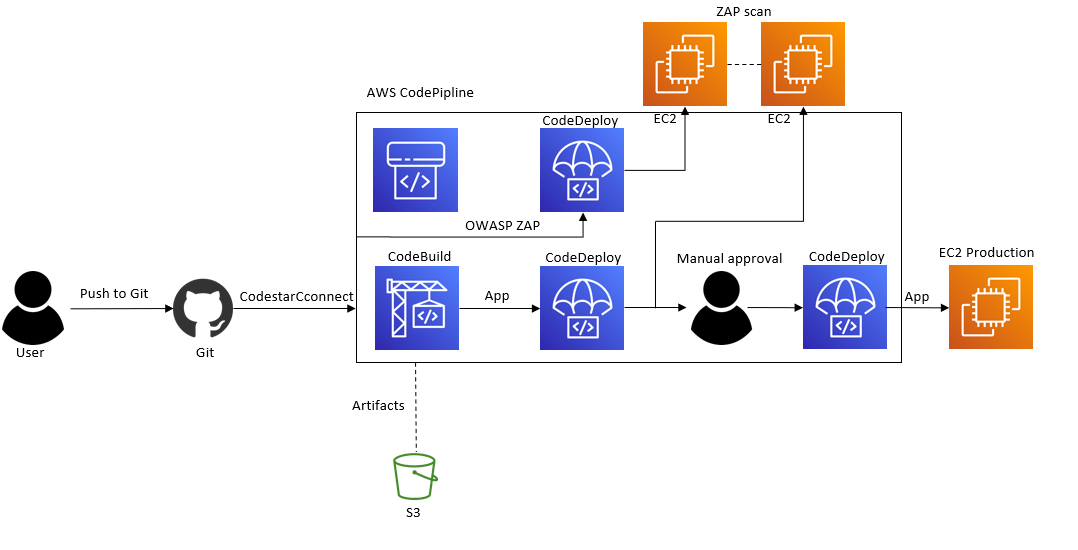
\includegraphics[width=0.8\columnwidth]{Images/aws-piplin-7.png}
    \caption{App depeploy}
    \label{fig: App depeploy}
\end{figure}